%!TEX root = ../report.tex
\subsection{Twitter Data} % (fold)
\label{sub:twitter_data}
Twitter is a web platform where users can post short messages with up to 140 characters to broadcast things they want the world to know. These messages are called \textit{tweets} and the whole Twitter system became very famous in the last years. That's the reason why there's a high interest in performing sentiment analysis on twitter data. We are provided with a set of 8000 tweets where each tweet was annotaded by 7 persons. Each one scored the given tweet on a range from $-5$ to $5$ (where $-5$ indicates a very negativ, $0$ a neutral and $5$ a positive sentiment). The highest and lowest rate were ignored and the average of the remaining 5 scores is given for every 8000 tweets. This data is provided by \textit{SemEval-2015 Task 11}.
% subsection twitter_data (end)

\subsection{Histogram} % (fold)
\label{sub:histogram}
In figure \ref{fig:hist_data} you can see, that the most tweets have a score next to negative 2

\begin{figure}[ht]
\centering 
  \begin{tabular}{@{}l@{}}
    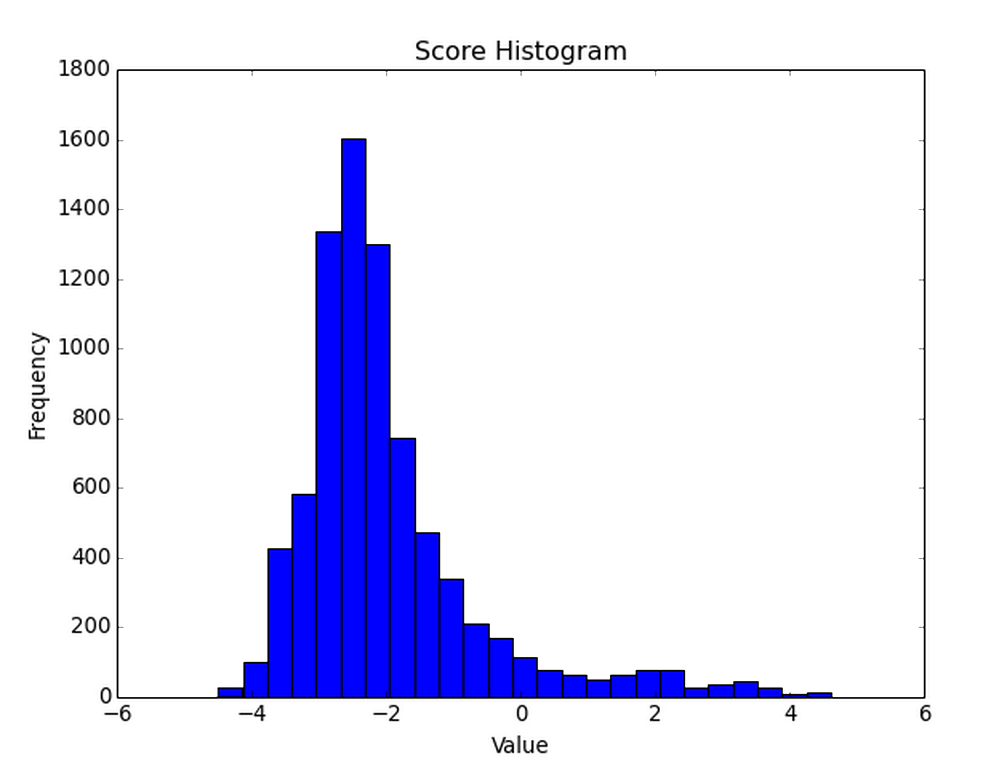
\includegraphics[width=0.6\linewidth]{img/data_hist.png}
  \end{tabular} 
  \caption{Histogram showing the score distribution for the given data} 
  \label{fig:hist_data} 
\end{figure}

% subsection histogram (end)

\subsection{Learning Task} % (fold)
\label{sub:learning_task}
yes
% subsection learning_task (end)

\subsection{Pipeline} % (fold)
\label{sub:pipeline}

% subsection pipeline (end)

\subsection{Evaluation} % (fold)
\label{sub:evaluation}

% subsection evaluation (end)